%!TEX root = cscw2019-comic.tex
\section{Study on Persuasion: Results}
\label{sec:Study on Behavior Results}

\subsection{Raw Data}
\label{sub:Study on Behavior Raw Data}
In total we have 307 participants joined our study, 101 participants received the message in the text form, 102 participants received the same message in the comic form, and 104 participants received the comic message with social-proof. We ran an outlier analysis on participants' completion time and removed 30 participants from our dataset. The following analysis is based on a dataset with 277 participants, 91 of them is in pure-text condition, 97 of them is in comic condition, and 92 of them is in comic-social-proof condition. Of those 277 participants, 150 were self-identified as male, and 126 were self-identified as female, 1 participant chose not to disclose. 197 participants earned at least college degree.

\begin{figure*}[htb]
	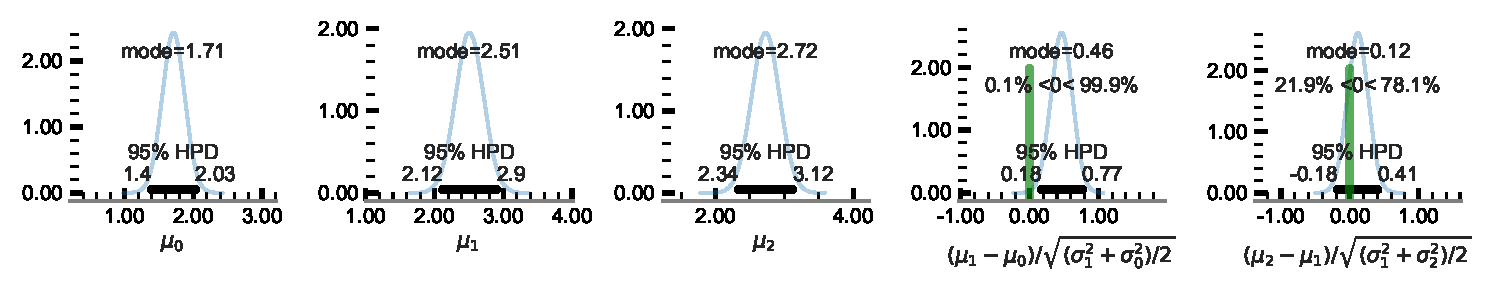
\includegraphics[width=1\textwidth]{./hari-code/new_exp_text_v_comic_v_social.pdf}
    \caption{The posterior distribution of the amount of money participants decide to donate to the charity in each of the three conditions: text only ($\mu_0$); comic ($\mu_1$); comic with social norm ($\mu_2$). The right two panels are respectively: posterior distribution of the effect size contrasting the comic condition ($\mu_1$) and text ($\mu_0$); the effect size contrasting comic with social norm ($\mu_2$) with the plain comic ($\mu_1$). First notice that $\mu_2 > \mu_1 > \mu_0$. Furthermore, the modal effect size of comparing the comic panel against text is 0.48, a medium effect and the HPD interval $[0.17, 0.77]$ reliably excludes a ROPE of $[0 \pm 0.1]$, indicating that the effect is meaningful. The effect of introducing the social norm into the comic has a minor effect (mode=0.12) when contrasted against the plan comic, and the HPD interval $[-0.17, 0.41]$ includes a ROPE of $[0 \pm 0.1]$, indicating that the outcome is not convincing.}
	\label{fig:main-experiment2-effect}
\end{figure*}

\subsection{Analysis}
\label{sub:Study on Behavior Analysis}

Now, we discuss our Bayesian formulation. There is one outcome variable $y_{i \mid j}$, the amount of donation to the charity by each participant $i$, under experimental condition $j$: text, comic, and comic with social norm. Our Bayesian model:

\begin{align}
    y_{i \mid j} \sim &  \mathrm{StudentT}(\nu, \mu_j, \sigma_j), \\
    \nu \sim & \exp(\lambda), \\
    \mu_j \sim & N(a,b), \\
    \sigma_j \sim & U(L,H).
\end{align}

We use a $\mathrm{StudentT}$ distribution with $\nu$ degrees of freedom to model the random variable; notice that this is a \textit{drawing distribution}, not the $t$-test. The $\mathrm{StudentT}$ allows us to model a non-Normal outcome with a heavy tail; assuming $y_{i \mid j}$ to be Normally distributed is equivalent to setting $\nu=\infty$. The degrees of freedom $\nu$ is drawn from an exponential distribution; the mode $\mu_j$ corresponding to each experimental group is drawn from a Normal distribution; the ``width'' $\sigma_j$ of the $t$-distribution corresponding to group $j$ is drawn from an uniform distribution. The hyper-priors for variables $\nu$, $\mu_j$ and $\sigma_j$ are set to be generous to allow for wide variation in these values. For example, we set $\lambda=\sfrac{1}/{29}$, since $\nu \geq 30$ is a rule of thumb for presence of Normality.

The result ~\Cref{fig:main-experiment2-effect} shows the modal effect size between abstract-comic v. pure-text = 0.48; There is no overlap of the 95\% high probability density (HPD) interval with the ROPE of [-0.1, 0.1]. Thus the effect is of medium size and meaningful; the effect size between abstract-comic and social-proof-comic is 0.12; but since the distribution includes a ROPE of $[-0.1 \pm 0.1]$, the effect is not convincing.

In this section, we presented a Bayesian model to analyze the overall effect of using a abstract-comic to persuade people making charitable donation decisions, and understand the effect of adapting persuasive techniques in the abstract comic form. The results show that the use of abstract-comic produces a significant effect in persuading participants to donate. Although abstract-comic with social proof can produce larger effect, the contrast between abstract-comic and abstract-comic with social proof is not significant. Next we discuss the findings, limitations and design implications.
